\documentclass[journal]{IEEEtran}
\IEEEoverridecommandlockouts
\usepackage{cite}
\usepackage{amsmath,amssymb,amsfonts}
\usepackage{amsthm}
\usepackage{bm}
\usepackage{graphicx}
\usepackage{booktabs}
\usepackage{multirow}
\usepackage{array}
\usepackage{algorithm}
\usepackage{algpseudocode}
\usepackage{url}
\usepackage{tikz}
\usetikzlibrary{arrows.meta,positioning,shapes.geometric,calc,fit,backgrounds,patterns}
\usepackage{pgfplots}
\usepgfplotslibrary{groupplots}
\pgfplotsset{compat=1.17}
\pgfplotsset{discard if not/.style 2 args={x filter/.append code={\edef\tempa{\thisrow{#1}}\edef\tempb{#2}\ifx\tempa\tempb\else\def\pgfmathresult{inf}\fi}}}
\usepackage{pgfplotstable}

\newtheorem{theorem}{Theorem}
\newtheorem{proposition}{Proposition}
\newtheorem{corollary}{Corollary}
\newtheorem{definition}{Definition}
\theoremstyle{remark}
\newtheorem{remark}{Remark}

\newcommand{\TabC}{Tabayyun-C}
\newcommand{\TabW}{Tabayyun-W}
\newcommand{\Mq}{\bm{M}^{\mathrm{Q}}}
\newcommand{\Mp}{\bm{M}^{\mathrm{P}}}
\newcommand{\Mpref}{\widetilde{\bm{M}}^{\mathrm{P}}}
\newcommand{\TrMean}{\operatorname{TrMean}}
\newcommand{\med}{\operatorname{med}}
\DeclareMathOperator*{\argmax}{arg\,max}
\makeatletter\newcommand\inputtab[1]{\@@input #1 }\makeatother

\tikzset{
  box/.style={draw, rectangle, minimum height=7mm, align=center, font=\footnotesize, inner sep=2pt},
  rbox/.style={draw, rectangle, rounded corners=2pt, minimum height=7mm, align=center, font=\footnotesize, inner sep=2pt},
  dbox/.style={draw, dashed, rectangle, minimum height=7mm, align=center, font=\footnotesize, inner sep=2pt},
  dec/.style={draw, diamond, aspect=2.2, align=center, font=\footnotesize, inner sep=0.5pt},
  term/.style={draw, rectangle, rounded corners=7pt, minimum height=6mm, align=center, font=\footnotesize, inner sep=2pt},
  arr/.style={-{Stealth[length=2.2mm]}, thick},
  darr/.style={-{Stealth[length=2.2mm]}, thick, dashed},
  lab/.style={font=\scriptsize, inner sep=1pt}
}

\begin{document}

\title{Witness-Optimal Certified Memory: Byzantine-Robust Test-Time Neural Memory With Runtime Certificates}

\author{Abraheem~Rashid, Faisal~Iradat, Waseem~Iqbal, Awais~Ahmad, Fakhri~Alam~Khan, and~Joel~Rodrigues%
\thanks{(Corresponding author: Waseem Iqbal, e-mail: m.waseem@squ.edu.om.)}%
\thanks{A. Rashid is with the Department of Computer Science, Brunel University London, London, U.K. (e-mail: 2546393@brunel.ac.uk).}%
\thanks{F. Iradat is with the Department of Computer Science, Institute of Business Administration, Karachi, Pakistan (e-mail: firadat@iba.edu.pk).}%
\thanks{W. Iqbal is with the Department of Electrical and Computer Engineering, Sultan Qaboos University, Muscat, Oman.}%
\thanks{A. Ahmad is with the Department of Cybersecurity and Cryptology, Faculty of Information Technology and Artificial Intelligence, Al-Farabi Kazakh National University, Almaty, Kazakhstan (e-mail: awais.ahmad@kaznu.edu.kz).}%
\thanks{F. A. Khan is with the Information and Computer Science Department, King Fahd University of Petroleum and Minerals, and the Interdisciplinary Research Center of Intelligent Secure Systems (IRC-ISS), King Fahd University of Petroleum and Minerals, Dhahran 31261, Saudi Arabia (e-mail: fakhri.khan@kfupm.edu.sa).}%
\thanks{J. Rodrigues is with the School of Information Science and Engineering, Zhejiang Sci-Tech University (ZSTU), China, and the Artificial Intelligence Research Center (AIRC), Ajman University, Ajman, United Arab Emirates (e-mail: joeljr@ieee.org).}}

\markboth{IEEE Transactions on Information Forensics and Security}%
{Rashid \MakeLowercase{\textit{et al.}}: Witness-Optimal Certified Memory}

\maketitle

\begin{abstract}
Test-time neural memories write every observed association into shared weights by a gradient step. When the associations come from several sources, a minority of compromised sources can install false facts, and the superposition of writes erases the provenance on which defences for retrieval stores rely. This paper presents Tabayyun, a two-tier memory in which each source writes into its own quarantine and an association enters the shared tier only after enough independent sources corroborate it. Promotion uses a trimmed mean over the corroborating sources and returns, at run time, a per-query bound on the deviation from the honest-source consensus that no other bound computed from the observed values can improve. The analysis establishes the witness complexity of the problem: agreement among f+1 sources is necessary and sufficient for bounded error, 2f+1 sources are necessary and sufficient for range validity, and neither threshold depends on the number of sources, whereas majority aggregation needs about half of them. Pre-registered experiments covered synthetic memories, trained memory language models, two frozen pretrained language models, federated clients and radio access network traces. No certificate violation occurred in 233,870 certified runs inside the threat model. Under union attacks combining gradient optimization with static attacks, the agreement-gated variant was installed on at most 5.0 percent of attacked facts, while gradient attacks installed up to 100 percent against the trimmed mean, and it recalled 32 to 34 points more locally held facts than the cone-gated variant. Sharding by key extends certification to 1,024 facts per memory.
\end{abstract}

\begin{IEEEkeywords}
Byzantine robustness, certified defense, data poisoning, federated learning, language model security, robust aggregation, test-time memory.
\end{IEEEkeywords}

%======================================================================
\section{Introduction}
\IEEEPARstart{L}{anguage} models with test-time memory update part of their parameters while they read. Titans~\cite{behrouz2024titans} and the Miras family~\cite{behrouz2025miras} store key--value associations in a neural memory through an online gradient step, in the line of fast-weight programmers~\cite{schlag2021linear} and test-time training~\cite{sun2024ttt}; federated variants share such memories across clients~\cite{chen2026fednl}. In deployment the written associations come from many sources: documents, tools, users and, in the federated case, other clients. A source that is compromised can therefore write into the same parameters that every later query reads.

Two lines of work address related threats, and neither covers this one. Byzantine-robust aggregation (trimmed mean and median~\cite{yin2018byzantine}, Krum~\cite{blanchard2017krum}, the geometric median~\cite{pillutla2022rfa}, centered clipping~\cite{karimireddy2021history}, FLTrust~\cite{cao2021fltrust}) combines whole updates and assumes that every honest participant holds the quantity being estimated. Defences for retrieval stores and agent memories (RobustRAG~\cite{xiang2024robustrag}, SMSR~\cite{sharma2026smsr}, origin-bound elevation~\cite{louck2026tma}) rely on items that keep their provenance. In a parametric memory both premises fail. Each fact is usually known to a few sources, so a majority rule discards it; and every write superposes into the same weights, so no item carries its origin.

This paper studies the problem formally and experimentally. Its central observation is that the relevant resource is the number of independent \emph{witnesses} of a fact, not the number of sources. A rule that counts witnesses can serve a fact known to a constant number of sources; a rule that takes a majority over all sources needs a number of witnesses that grows with the population.

The contributions are as follows.
\begin{enumerate}
\item \emph{A two-tier memory with per-source quarantine and corroborated promotion} (Section~\ref{sec:method}). Writes enter only the writer's quarantine; a direction of key space is promoted to a shared, linear, momentum-free tier when $k$ sources corroborate it, with a cone gate ($k=2f+1$, \TabC) or an agreement gate ($k=f+1$, \TabW).
\item \emph{Runtime certificates} (Section~\ref{sec:theory}). The promoted tier carries a per-direction error that bounds, for every query, the deviation from the honest-source consensus, together with a token-level action certificate. The order-statistic bound is the smallest sound bound computable from the observed values (Theorem~\ref{thm:opt}).
\item \emph{Witness complexity} (Theorem~\ref{thm:witness}). $f+1$ agreeing witnesses are necessary and sufficient for bounded error, $2f+1$ are necessary and sufficient for coordinate-wise range validity, and both thresholds are independent of the population size $n$; majority aggregation requires more than $n/2$ witnesses.
\item \emph{A pre-registered evaluation} (Sections~\ref{sec:setup}--\ref{sec:results}) on five substrates, with static, gradient-based and union attackers, 18 registered amendments, and failures reported as failures.
\end{enumerate}
The name \emph{tabayyun} denotes, in Arabic, the verification of a report before acting on it. Section~\ref{sec:related} reviews related work, Section~\ref{sec:model} defines the system and threat model, Section~\ref{sec:discussion} states the limitations and Section~\ref{sec:conclusion} concludes.

%======================================================================
\section{Related Work}\label{sec:related}
\emph{Poisoning and Byzantine-robust learning.} Data poisoning was studied for support vector machines~\cite{biggio2012poisoning} and later for distributed and federated training. Robust aggregators bound the influence of $f$ faulty updates~\cite{yin2018byzantine,blanchard2017krum,pillutla2022rfa,karimireddy2021history,cao2021fltrust}, and optimized attacks show that their guarantees are loose in high dimension~\cite{fang2020local,baruch2019little,shejwalkar2021manipulating}. Certified defences bound the effect of poisoned training data~\cite{steinhardt2017certified,jia2021bagging,levine2021dpa} or of poisoned clients~\cite{cao2022flcert}; privacy-preserving variants appear in~\cite{ma2022shieldfl,liu2021privacy}. These methods aggregate full updates under an honest majority over all participants.

\emph{Memory and retrieval poisoning.} PoisonedRAG~\cite{zou2025poisonedrag} and AgentPoison~\cite{chen2024agentpoison} corrupt retrieval stores and agent memories. RobustRAG~\cite{xiang2024robustrag} isolates each retrieved passage and aggregates the answers; SMSR~\cite{sharma2026smsr} certifies by randomized ablation and voting; origin-bound authority~\cite{louck2026tma} elevates a memory item only after Sybil-resistant corroboration and binds authority to the write-time origin. All three operate on discrete items with provenance.

\emph{Test-time memory.} Titans~\cite{behrouz2024titans}, Miras~\cite{behrouz2025miras} and test-time training layers~\cite{sun2024ttt} update a memory by online regression; federated nested learning~\cite{chen2026fednl} averages such memories across clients. No security mechanism is specified for them.

\emph{Byzantine agreement.} Byzantine agreement~\cite{lamport1982byzantine} and approximate agreement on real values~\cite{dolev1986approximate} tolerate $f$ faulty processes, and a client of a replicated service accepts a result after $f+1$ matching replies~\cite{castro1999pbft}. Vector consensus with convex-hull validity needs a number of processes that grows with the dimension~\cite{vaidya2013vector,mendes2013multidimensional}. Theorem~\ref{thm:witness} uses the weaker coordinate-wise range validity, for which the requirement does not depend on the dimension, and adds a runtime error bound. Table~\ref{tab:position} positions the method.

\begin{table}[!t]
\caption{Positioning by Method Class ($\checkmark$: Provided; --: Not Provided)}
\label{tab:position}
\centering\footnotesize
\setlength{\tabcolsep}{3pt}
\resizebox{\columnwidth}{!}{%
\begin{tabular}{@{}lccccc@{}}
\toprule
Class & Param. & Per-source & Witnesses & Runtime & Adaptive \\
 & memory & isolation & needed & bound & attack \\
\midrule
Robust aggregation~\cite{yin2018byzantine,blanchard2017krum,pillutla2022rfa} & $\checkmark$ & -- & $>n/2$ & -- & \cite{fang2020local,shejwalkar2021manipulating} \\
Certified poisoning~\cite{jia2021bagging,levine2021dpa,cao2022flcert} & -- & partition & vote & $\checkmark$ & -- \\
Retrieval / agent memory~\cite{xiang2024robustrag,sharma2026smsr} & -- & $\checkmark$ & majority & $\checkmark$ & -- \\
Origin-bound elevation~\cite{louck2026tma} & -- & $\checkmark$ & $k$ & -- & -- \\
Test-time memory~\cite{behrouz2024titans,chen2026fednl} & $\checkmark$ & -- & -- & -- & -- \\
\midrule
\TabC\ / \TabW\ (this paper) & $\checkmark$ & $\checkmark$ & $2f{+}1$ / $f{+}1$ & $\checkmark$ & $\checkmark$ \\
\bottomrule
\end{tabular}}
\end{table}

%======================================================================
\section{System and Threat Model}\label{sec:model}
Table~\ref{tab:notation} lists the notation.

\begin{table}[!t]
\caption{Notation}
\label{tab:notation}
\centering\footnotesize
\setlength{\tabcolsep}{4pt}
\begin{tabular}{@{}ll@{}}
\toprule
Symbol & Meaning \\
\midrule
$n,\ f$ & Number of sources; tolerated Byzantine sources \\
$m$ & Honest witnesses of a fact \\
$\rho,\ R$ & Observation probability per round; rounds \\
$\Mq_s$ & Quarantine memory of source $s$ \\
$\Mp,\ \Mpref$ & Promoted tier; its honest reference \\
$\bm{U},\ \bm{u}$ & Anchored basis; one direction \\
$\bm{D}_{s,u}$ & Read of source $s$ along $\bm{u}$ \\
$A_u,\ C_u$ & Active sources; corroborators of $\bm{u}$ \\
$k,\ \beta_u$ & Promotion threshold; trimming per side \\
$\gamma,\ \epsilon$ & Cone angle; agreement tolerance \\
$\bm{x}_u,\ \bm{e}_u$ & Promoted value; its runtime error \\
$\bm{E}_u,\ b(\bm{q})$ & Drift certificate; per-query bound \\
$F,\ S$ & Facts per memory; number of shards \\
\bottomrule
\end{tabular}
\end{table}

\subsection{Memory Model}
A linear memory $\bm{M}\in\mathbb{R}^{d_v\times d_k}$ answers a query $\bm{q}$ with $\bm{y}=\bm{M}\bm{q}$. A write of the pair $(\bm{k}_t,\bm{v}_t)$ follows the Titans update~\cite{behrouz2024titans}
\begin{equation}\label{eq:titans}
\begin{aligned}
\bm{S}_t&=\eta\bm{S}_{t-1}-\theta\,\nabla_{\bm{M}}\|\bm{M}_{t-1}\bm{k}_t-\bm{v}_t\|_2^2,\\
\bm{M}_t&=(1-\alpha)\bm{M}_{t-1}+\bm{S}_t,
\end{aligned}
\end{equation}
with momentum $\eta$, step $\theta$ and forget gate $\alpha$. In a shared memory all writes enter the same $\bm{M}$.

\subsection{Sources, Adversary and Goals}
There are $n$ sources $s\in[n]$; at most $f$ are Byzantine and their identities are unknown. A fact $(\bm{k}_j,\bm{v}_j)$ is known to a set $H_j$ of $m_j=|H_j|$ honest sources (its \emph{witnesses}), each of which observes it with probability $\rho$ in each of $R$ observation rounds. Facts known to all honest sources form the \emph{dense} regime; facts known to a minority form the \emph{locality} regime.

The adversary is white-box: it knows the memory, the gate, its parameters and every honest quarantine. Its sources may write any sequence of pairs; in the adaptive attacks of Section~\ref{sec:setup} it sets the states of its own quarantines directly. Its goal is to \emph{install} a target value $\bm{v}^\star$ at a key $\bm{k}^\star$, that is, to make the memory return $\bm{v}^\star$ (for a language model, the attacker's token), or to cause \emph{amnesia} of the true value. Honest sources are assumed independent: the adversary does not control what they observe. Section~\ref{sec:limits} measures what happens when this assumption fails.

\subsection{Reference and Metrics}
Let $\Mpref$ be the promoted memory that would result if every promoted value were replaced by the mean of the honest corroborators, under the same promotion decisions. A certificate is \emph{sound} if it upper-bounds $\|(\Mp-\Mpref)\bm{q}\|$ for the queries it covers. The metrics are clean recall, installed rate, amnesia rate, the fraction of tokens that are certified and correct, and the \emph{served-installed} rate under certify-or-abstain serving (Section~\ref{sec:serving}).

%======================================================================
\section{Method}\label{sec:method}
Fig.~\ref{fig:arch} shows the architecture. The write path keeps sources apart; the promotion path decides what enters the shared tier and with what error; the read path answers queries and attaches a certificate.

\begin{figure*}[!t]
\centering
\resizebox{\textwidth}{!}{%
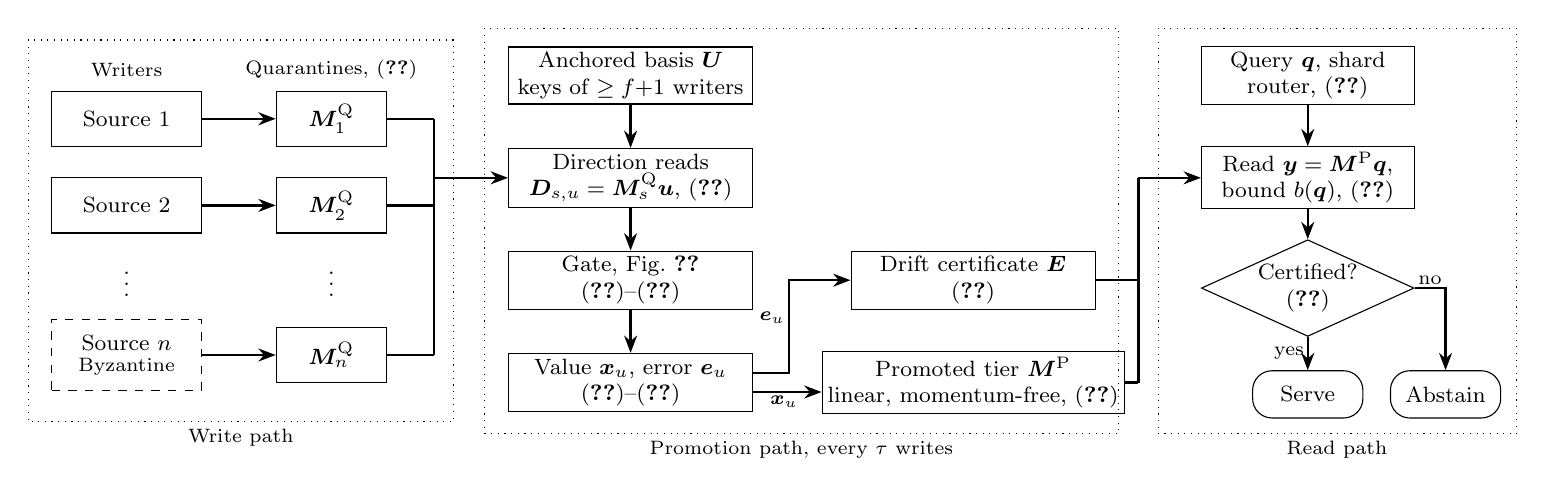
\begin{tikzpicture}[x=1cm,y=1cm]
% ---------------- write path
\node[box, minimum width=19mm] (s1) at (0,0) {Source $1$};
\node[box, minimum width=19mm] (s2) at (0,-1.1) {Source $2$};
\node[font=\footnotesize] at (0,-2.0) {$\vdots$};
\node[dbox, minimum width=19mm, minimum height=9mm] (sn) at (0,-3.0) {Source $n$\\[-2pt]{\scriptsize Byzantine}};
\node[box, minimum width=14mm] (q1) at (2.6,0) {$\Mq_1$};
\node[box, minimum width=14mm] (q2) at (2.6,-1.1) {$\Mq_2$};
\node[font=\footnotesize] at (2.6,-2.0) {$\vdots$};
\node[box, minimum width=14mm] (qn) at (2.6,-3.0) {$\Mq_n$};
\node[lab] at (0,0.62) {Writers};
\node[lab] at (2.6,0.62) {Quarantines, (\ref{eq:titans})};
\draw[arr] (s1) -- (q1);
\draw[arr] (s2) -- (q2);
\draw[arr] (sn) -- (qn);
\draw[thick] (q1.east) -- (3.9,0);
\draw[thick] (q2.east) -- (3.9,-1.1);
\draw[thick] (qn.east) -- (3.9,-3.0);
\draw[thick] (3.9,0) -- (3.9,-3.0);
% ---------------- promotion path
\node[box, minimum width=31mm] (basis) at (6.4,0.55) {Anchored basis $\bm{U}$\\keys of $\ge f{+}1$ writers};
\node[box, minimum width=31mm] (reads) at (6.4,-0.75) {Direction reads\\$\bm{D}_{s,u}=\Mq_s\bm{u}$, (\ref{eq:reads})};
\node[box, minimum width=31mm] (gate) at (6.4,-2.05) {Gate, Fig.~\ref{fig:gate}\\(\ref{eq:active})--(\ref{eq:agree})};
\node[box, minimum width=31mm] (val) at (6.4,-3.35) {Value $\bm{x}_u$, error $\bm{e}_u$\\(\ref{eq:value})--(\ref{eq:err})};
\node[box, minimum width=31mm] (cert) at (10.75,-2.05) {Drift certificate $\bm{E}$\\(\ref{eq:drift})};
\node[box, minimum width=31mm] (promo) at (10.75,-3.35) {Promoted tier $\Mp$\\linear, momentum-free, (\ref{eq:ema})};
\draw[arr] (3.9,-0.75) -- (reads.west);
\draw[arr] (basis) -- (reads);
\draw[arr] (reads) -- (gate);
\draw[arr] (gate) -- (val);
\draw[arr] ([yshift=-1.2mm]val.east) -- node[lab, below, pos=0.45]{$\bm{x}_u$} ([yshift=-1.2mm]promo.west);
\draw[arr] ([yshift=1.2mm]val.east) -- ++(0.45,0) |- node[lab, left, pos=0.3]{$\bm{e}_u$} (cert.west);
% ---------------- read path
\node[box, minimum width=27mm] (route) at (15.0,0.55) {Query $\bm{q}$, shard\\router, (\ref{eq:shard})};
\node[box, minimum width=27mm] (readq) at (15.0,-0.75) {Read $\bm{y}=\Mp\bm{q}$,\\bound $b(\bm{q})$, (\ref{eq:qbound})};
\node[dec] (ok) at (15.0,-2.15) {Certified?\\(\ref{eq:action})};
\node[term, minimum width=14mm] (serve) at (15.0,-3.5) {Serve};
\node[term, minimum width=14mm] (abst) at (16.75,-3.5) {Abstain};
\draw[arr] (route) -- (readq);
\draw[arr] (readq) -- (ok);
\draw[arr] (ok.south) -- node[lab, left]{yes} (serve.north);
\draw[arr] (ok.east) -| node[lab, above, pos=0.25]{no} (abst.north);
\draw[thick] (promo.east) -- (12.85,-3.35);
\draw[thick] (cert.east) -- (12.85,-2.05);
\draw[thick] (12.85,-3.35) -- (12.85,-0.75);
\draw[arr] (12.85,-0.75) -- (readq.west);
% ---------------- bands
\draw[dotted] (-1.25,1.0) rectangle (4.15,-3.85);
\draw[dotted] (4.55,1.15) rectangle (12.6,-4.0);
\draw[dotted] (13.1,1.15) rectangle (17.65,-4.0);
\node[lab, anchor=north] at (1.45,-3.9) {Write path};
\node[lab, anchor=north] at (8.57,-4.05) {Promotion path, every $\tau$ writes};
\node[lab, anchor=north] at (15.37,-4.05) {Read path};
\end{tikzpicture}}
\caption{Architecture of Tabayyun. Each source writes only into its own quarantine. Every $\tau$ writes, the quarantines are read along an anchored basis, a gate selects the corroborating sources of each direction, and the trimmed value and its runtime error update the promoted tier and the drift certificate. A query is routed to its shard, read from the promoted tier and answered only if the answer is certified. The dashed box marks a Byzantine source; numbers in parentheses refer to equations.}
\label{fig:arch}
\end{figure*}

\subsection{Quarantine and Anchored Basis}
Source $s$ writes only into its quarantine $\Mq_s$, updated by (\ref{eq:titans}) with step $\theta$ and forget gate $\alpha^{\mathrm{Q}}$. Every $\tau$ writes a promotion round reads the quarantines along an orthonormal basis $\bm{U}=[\bm{u}_1,\dots,\bm{u}_K]^{\top}$:
\begin{equation}\label{eq:reads}
\bm{D}_{s,u}=\Mq_s\bm{u}\in\mathbb{R}^{d_v},\qquad s\in[n],\ u\in\bm{U}.
\end{equation}
A direction is added to $\bm{U}$, and then frozen, when a key has been written by at least $f+1$ distinct sources; this \emph{anchored} basis aligns each direction with one fact. Frozen directions keep the certificate of Section~\ref{sec:theory} well defined.

\subsection{Active Set and Corroborators}
Let $\sigma_u$ be the $(f+1)$-th largest norm $\|\bm{D}_{s,u}\|$. Since at most $f$ norms are adversarial, $\sigma_u$ never exceeds the largest honest norm. The active set is
\begin{equation}\label{eq:active}
A_u=\{s:\|\bm{D}_{s,u}\|\ge\max(\nu,\ \nu_{\mathrm{rel}}\,\sigma_u)\}.
\end{equation}
The relative threshold removes the small cross-talk reads that non-orthogonal keys leave in sources that never wrote the fact.

\emph{Cone gate} (\TabC). With $\bm{m}_u$ the coordinate-wise median over $A_u$, the corroborators are
\begin{equation}\label{eq:cone}
C_u=\{s\in A_u:\cos(\bm{D}_{s,u},\bm{m}_u)\ge\gamma\},\qquad k=2f+1.
\end{equation}

\emph{Agreement gate} (\TabW). With the ball $B_u(c)=\{s\in A_u:\|\bm{D}_{s,u}-\bm{D}_{c,u}\|_2\le\epsilon\sigma_u\}$, the corroborators are the most populated ball (ties broken by the smaller total distance):
\begin{equation}\label{eq:agree}
C_u=B_u(c^\star),\quad c^\star=\argmax_{c\in A_u}|B_u(c)|,\qquad k=f+1.
\end{equation}

\subsection{Promotion and Runtime Error}
Direction $u$ is promoted if $|C_u|\ge k$. Its value is the coordinate-wise trimmed mean over the corroborators,
\begin{equation}\label{eq:value}
\begin{aligned}
\bm{x}_u&=\TrMean_{\beta_u}\{\bm{D}_{s,u}:s\in C_u\},\\
\beta_u&=\min\big(f,\ \lfloor(|C_u|-1)/2\rfloor\big),
\end{aligned}
\end{equation}
which removes $\beta_u$ values from each end of every coordinate. Let $c=|C_u|$ and, for coordinate $i$, let $L_{u,i}$ and $U_{u,i}$ be the means of the $c-f$ smallest and the $c-f$ largest corroborator values. The runtime error is
\begin{equation}\label{eq:err}
e_{u,i}=\begin{cases}\max\big(x_{u,i}-L_{u,i},\,U_{u,i}-x_{u,i}\big), & c\ge 2f{+}1,\\[2pt]
\max\big(x_{u,i}-\underline{x}_{u,i},\,\overline{x}_{u,i}-x_{u,i}\big), & \text{otherwise},\end{cases}
\end{equation}
where $\underline{x}_{u,i}$ and $\overline{x}_{u,i}$ are the smallest and largest corroborator values in coordinate $i$.
The promoted tier is updated by a convex step, and the drift certificate follows the same recursion:
\begin{align}
\Mp&\leftarrow\Mp+\alpha_{\mathrm{P}}\textstyle\sum_{u\ \mathrm{promoted}}(\bm{x}_u-\Mp\bm{u})\bm{u}^{\top},\label{eq:ema}\\
E_{u,i}&\leftarrow(1-\alpha_{\mathrm{P}})E_{u,i}+\alpha_{\mathrm{P}}e_{u,i}\quad(u\ \mathrm{promoted}).\label{eq:drift}
\end{align}
The promoted tier has no momentum. Section~\ref{sec:ablation} shows that adding momentum to (\ref{eq:ema}) invalidates the certificate.

\begin{figure}[!t]
\centering
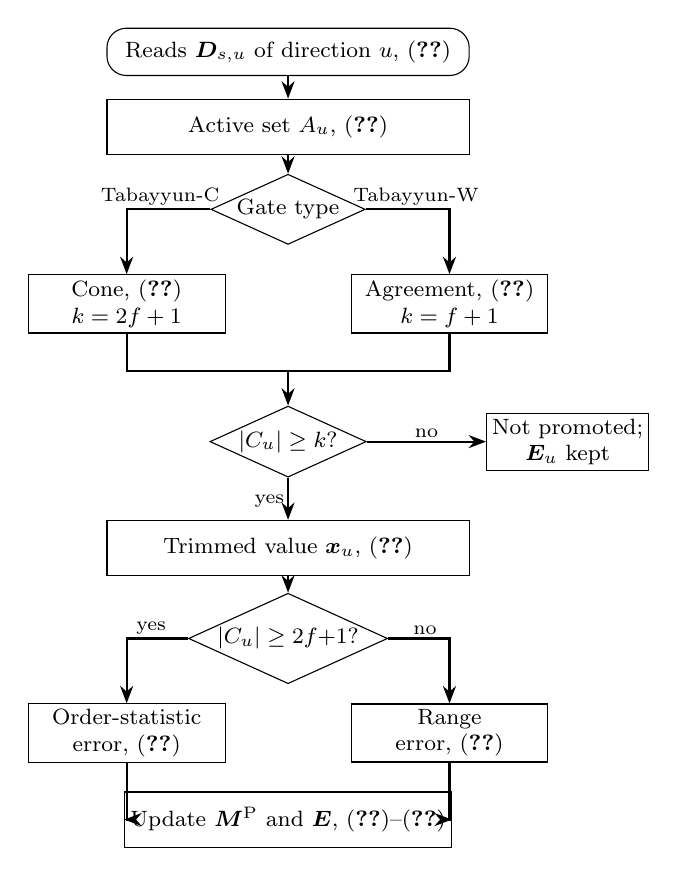
\begin{tikzpicture}[x=1cm,y=1cm]
\node[term, minimum width=46mm] (in) at (3.4,0) {Reads $\bm{D}_{s,u}$ of direction $u$, (\ref{eq:reads})};
\node[box, minimum width=46mm] (act) at (3.4,-0.95) {Active set $A_u$, (\ref{eq:active})};
\node[dec] (rule) at (3.4,-2.0) {Gate type};
\node[box, minimum width=25mm] (cone) at (1.35,-3.2) {Cone, (\ref{eq:cone})\\$k=2f+1$};
\node[box, minimum width=25mm] (agr) at (5.45,-3.2) {Agreement, (\ref{eq:agree})\\$k=f+1$};
\coordinate (mrg) at (3.4,-4.05);
\node[dec] (cnt) at (3.4,-4.95) {$|C_u|\ge k$?};
\node[box, minimum width=17mm] (np) at (6.95,-4.95) {Not promoted;\\$\bm{E}_u$ kept};
\node[box, minimum width=46mm] (val) at (3.4,-6.3) {Trimmed value $\bm{x}_u$, (\ref{eq:value})};
\node[dec] (big) at (3.4,-7.45) {$|C_u|\ge 2f{+}1$?};
\node[box, minimum width=25mm] (pr) at (1.35,-8.65) {Order-statistic\\error, (\ref{eq:err})};
\node[box, minimum width=25mm] (rr) at (5.45,-8.65) {Range\\error, (\ref{eq:err})};
\node[box, minimum width=30mm] (upd) at (3.4,-9.75) {Update $\Mp$ and $\bm{E}$, (\ref{eq:ema})--(\ref{eq:drift})};
\draw[arr] (in) -- (act);
\draw[arr] (act) -- (rule);
\draw[arr] (rule.west) -| node[lab, above, pos=0.3]{\TabC} (cone.north);
\draw[arr] (rule.east) -| node[lab, above, pos=0.3]{\TabW} (agr.north);
\draw[thick] (cone.south) |- (mrg);
\draw[thick] (agr.south) |- (mrg);
\draw[arr] (mrg) -- (cnt.north);
\draw[arr] (cnt.east) -- node[lab, above]{no} (np.west);
\draw[arr] (cnt.south) -- node[lab, left, pos=0.55]{yes} (val.north);
\draw[arr] (val) -- (big);
\draw[arr] (big.west) -| node[lab, above, pos=0.3]{yes} (pr.north);
\draw[arr] (big.east) -| node[lab, above, pos=0.3]{no} (rr.north);
\draw[arr] (pr.south) |- (upd.west);
\draw[arr] (rr.south) |- (upd.east);
\end{tikzpicture}
\caption{Promotion of one direction $u$. The cone gate requires $2f+1$ corroborators and keeps the value inside the honest range; the agreement gate requires $f+1$ corroborators that agree within $\epsilon\sigma_u$ and bounds the shift by $2\epsilon\sigma_u$. The error is the order-statistic error when at least $2f+1$ sources corroborate and the range error otherwise.}
\label{fig:gate}
\end{figure}

\subsection{Certified Serving and Sharding}\label{sec:serving}
For a query $\bm{q}$, the deviation of the read from the reference read is bounded per coordinate and in norm by
\begin{equation}\label{eq:qbound}
b(\bm{q})=\Big\|\textstyle\sum_{u}|\langle\bm{u},\bm{q}\rangle|\,\bm{E}_{u}\Big\|_2\ \ge\ \|(\Mp-\Mpref)\bm{q}\|_2 .
\end{equation}
When the read enters a linear head $\bm{z}=\bm{W}\bm{y}+\bm{c}$ (for a language model, $\bm{W}=g\bm{W}_U$ with unembedding $\bm{W}_U$ and read gain $g$), the predicted token $a=\arg\max_j z_j$ is certified if
\begin{equation}\label{eq:action}
z_a-z_j>\|\bm{w}_a-\bm{w}_j\|_2\,b(\bm{q})\qquad\forall j\ne a,
\end{equation}
because no read within $b(\bm{q})$ of $\bm{y}$ can change the arg max. For a linear utility $u_a=\bm{w}^{\top}\bm{y}_a$ over actions, the regret of the chosen action $\hat{a}$ under the reference is at most
\begin{equation}\label{eq:regret}
\hat{\varepsilon}=\max_j\big(u_j-u_{\hat a}+s_j+s_{\hat a}\big)^{+},\qquad s_a=\textstyle\sum_i|w_i|\,B_{a,i},
\end{equation}
with $B_{a,i}$ the per-coordinate bound of (\ref{eq:qbound}). Under \emph{certify-or-abstain} serving, the memory answers only when (\ref{eq:action}) holds.

The certificate degrades when one memory holds many facts, because interference between near-orthogonal keys makes honest quarantines disagree (Section~\ref{sec:scale}). Sharding removes this limit. A key is routed to one of $S$ independent instances by
\begin{equation}\label{eq:shard}
\mathrm{shard}(\bm{k})=\argmax_{j\in[S]}\ \langle\bm{p}_j,\bm{k}\rangle,
\end{equation}
with fixed random projections $\bm{p}_j$. Writers and readers route identically, so every shard is a complete instance and all results of Section~\ref{sec:theory} hold per shard and per query. Algorithm~\ref{alg:round} summarizes one promotion round and the serving rule.

\begin{algorithm}[!t]
\caption{Promotion Round and Certified Serving}
\label{alg:round}
\begin{algorithmic}[1]
\Require quarantines $\{\Mq_s\}_{s\in[n]}$, basis $\bm{U}$, parameters $f,k,\gamma,\epsilon,\nu,\nu_{\mathrm{rel}},\alpha_{\mathrm{P}}$
\For{each direction $\bm{u}\in\bm{U}$}
  \State $\bm{D}_{s,u}\gets\Mq_s\bm{u}$ for every $s\in[n]$ \Comment{(\ref{eq:reads})}
  \State $A_u\gets$ active sources \Comment{(\ref{eq:active})}
  \State $C_u\gets$ corroborators \Comment{(\ref{eq:cone}) or (\ref{eq:agree})}
  \If{$|C_u|\ge k$}
    \State $\bm{x}_u,\bm{e}_u\gets$ value and error \Comment{(\ref{eq:value}), (\ref{eq:err})}
    \State update $\Mp$ and $\bm{E}_u$ \Comment{(\ref{eq:ema}), (\ref{eq:drift})}
  \EndIf
\EndFor
\Function{Serve}{$\bm{q}$}
  \State route $\bm{q}$ to its shard \Comment{(\ref{eq:shard})}
  \State $\bm{y}\gets\Mp\bm{q}$; compute $b(\bm{q})$ \Comment{(\ref{eq:qbound})}
  \If{(\ref{eq:action}) holds for $a=\arg\max_j z_j$}
    \State \Return $a$
  \Else
    \State \Return abstain
  \EndIf
\EndFunction
\end{algorithmic}
\end{algorithm}

\emph{Cost.} With $K$ directions, a round costs
\begin{equation}\label{eq:cost}
T_{\mathrm{round}}=\begin{cases}O\big(nKd_vd_k+Kd_v\,n\log n\big), & \text{cone gate},\\
O\big(nKd_vd_k+Kd_v\,n^2\big), & \text{agreement gate},\end{cases}
\end{equation}
dominated by the reads (\ref{eq:reads}) for $n\ll d_k$; the per-query bound costs $O(Kd_v)$, and the action certificate costs $O(Vd_v)$ for a vocabulary of $V$ tokens when the pairwise distances in (\ref{eq:action}) are computed from the Gram identity $\|\bm{w}_a-\bm{w}_j\|_2^2=\|\bm{w}_a\|_2^2+\|\bm{w}_j\|_2^2-2\bm{w}_a^{\top}\bm{w}_j$.

%======================================================================
\section{Theoretical Guarantees}\label{sec:theory}
Each statement is followed by its proof. Throughout, $f$ is the number of Byzantine sources that the gate is configured to tolerate.

\begin{theorem}[Runtime certificate]\label{thm:cert}
Fix a promoted direction $u$ and a coordinate $i$, and let at most $f$ of the $c=|C_u|$ corroborators be Byzantine. Let $\mu_{u,i}$ be the mean of the honest corroborators. Then $|x_{u,i}-\mu_{u,i}|\le e_{u,i}$ with $e_{u,i}$ as in (\ref{eq:err}). Consequently $|(\Mp-\Mpref)\bm{u}|_i\le E_{u,i}$ after every round, and (\ref{eq:qbound}) holds for every query.
\end{theorem}
\begin{proof}
If $c\ge 2f+1$, the honest set has $h\ge c-f$ elements; the mean of any $h$ of the sorted values is at least the mean of the $c-f$ smallest and at most the mean of the $c-f$ largest, so $\mu_{u,i}\in[L_{u,i},U_{u,i}]$. If $f+1\le c\le 2f$, at least one corroborator is honest, so $\mu_{u,i}\in[\underline{x}_{u,i},\overline{x}_{u,i}]$. In both cases the distance from $x_{u,i}$ to $\mu_{u,i}$ is at most the distance to the farther end of the interval. The recursion (\ref{eq:ema}) applied to $\Mp-\Mpref$ along $\bm{u}$ is a convex combination of the previous deviation and $x_{u,i}-\tilde{x}_{u,i}$, which gives (\ref{eq:drift}); (\ref{eq:qbound}) follows from the triangle inequality over $\bm{q}=\sum_u\langle\bm{u},\bm{q}\rangle\bm{u}$.
\end{proof}

\begin{theorem}[Instance optimality]\label{thm:opt}
For $c\ge 2f+1$, every bound $B(\cdot)$ that is computed from the observed corroborator values and is sound for every placement of at most $f$ Byzantine values satisfies $B\ge e_{u,i}$.
\end{theorem}
\begin{proof}
For an observed vector of values, both ``the $c-f$ smallest values are honest'' and ``the $c-f$ largest values are honest'' are consistent with the threat model. In these two worlds $\mu_{u,i}=L_{u,i}$ and $\mu_{u,i}=U_{u,i}$, while the observation, and hence $x_{u,i}$ and $B$, are identical. Soundness in both worlds requires $B\ge\max(x_{u,i}-L_{u,i},\,U_{u,i}-x_{u,i})=e_{u,i}$.
\end{proof}

\begin{theorem}[Witness complexity]\label{thm:witness}
Consider one direction with $c$ active reports, at most $f$ of them Byzantine.
\begin{enumerate}
\item[(a)] A rule whose output is within a bound of some honest report that the adversary cannot enlarge must abstain whenever $c\le f$.
\item[(b)] If at least $f+1$ active reports lie within $r=\epsilon\sigma_u$ of one of them, every point $\bm{x}$ of their coordinate-wise range satisfies $\|\bm{x}-\bm{h}\|_\infty\le 2r$ for an honest report $\bm{h}$ among them, and $r$ is at most $\epsilon$ times the largest honest norm.
\item[(c)] Coordinate-wise range validity, $\min_H\le x_i\le\max_H$ for every $i$, requires abstention for some inputs with $c\le 2f$, and the trimmed mean with $\beta=f$ achieves it for every input with $c\ge 2f+1$.
\item[(d)] Let $m$ honest sources know a fact with positive value $v$ in coordinate $i$, let the other $n-m$ sources report $0$ (silent adversaries included), and let $m>f$. The coordinate median over all $n$ sources returns $0$ when $m<n/2$, and the trimmed mean with $\beta=f$ returns $\frac{m-f}{n-2f}v\le v/2$ when $m\le n/2$.
\end{enumerate}
\end{theorem}
\begin{proof}
(a) With $c\le f$ all reports may be Byzantine, so no honest report needs to exist. (b) A set of $f+1$ reports contains an honest report $\bm{h}$; every member lies within $r$ of the centre and hence within $2r$ of $\bm{h}$ in $\ell_2$ and in each coordinate, and the coordinate-wise range inherits the coordinate bound. At most $f$ norms are adversarial, so the $(f+1)$-th largest norm is at most the largest honest norm. (c) For $c=2f$, place $f$ reports at $\bm{a}$ and $f$ at $\bm{b}\ne\bm{a}$. Either half may be the honest one, the input is the same, and the two honest ranges $\{\bm{a}\}$ and $\{\bm{b}\}$ are disjoint, so no output is valid in both worlds. Sufficiency: every value below the honest minimum is Byzantine, there are at most $f\le\beta$ of them, and all are trimmed; the same holds above. (d) With $m<n/2$ nonzero values the median is $0$. Sorting $n$ values with $n-m$ zeros and trimming $f$ from each end leaves $m-f$ copies of the honest values among $n-2f$ retained values, and $(m-f)/(n-2f)\le 1/2$ when $m\le n/2$.
\end{proof}

\begin{corollary}[Recall law]\label{cor:recall}
If the adversaries stay silent on a fact and each of its $m$ witnesses observes it with probability $p_R=1-(1-\rho)^R$ over $R$ rounds, the probability that a gate with threshold $k$ promotes the fact, given that at least one witness observed it, is
\begin{equation}\label{eq:recall}
\Pr[\text{promoted}]=\frac{\Pr[\mathrm{Bin}(m,p_R)\ge k]}{\Pr[\mathrm{Bin}(m,p_R)\ge 1]},
\end{equation}
with $k=f+1$ for \TabW\ and $k=2f+1$ for \TabC.
For $k=f+1$, Theorem~\ref{thm:witness}(a) implies that no rule with bounded error has a larger promotion probability when the adversaries are silent.
\end{corollary}

\begin{remark}[Federated composition]
In the two-level federated form, each client reports its promoted reads $\bm{D}_c=\Mp_c\bm{u}$ and a local bound $\delta_c(\bm{u})=\sum_v|\langle\bm{v},\bm{u}\rangle|\bm{E}^c_v$, and the server applies the gate across clients. The global error is
\begin{equation}\label{eq:fed}
\bm{e}^{\mathrm{G}}_u=\bm{e}^{\mathrm{server}}_u+\max_{c\in[N]}\delta_c(\bm{u}),
\end{equation}
which remains sound when Byzantine clients under-report their bounds, because the maximum over all reports includes every honest report.
\end{remark}

%======================================================================
\section{Experimental Setup}\label{sec:setup}
\subsection{Substrates and Data}
Table~\ref{tab:setup} lists the five substrates. \emph{Tier A} uses synthetic facts with orthonormal keys ($d_k=d_v=32$). \emph{Tier B} uses memory language models with a Titans scan, trained on multi-query associative recall (MQAR) following the Zoology protocol~\cite{arora2024zoology}, at three sizes. \emph{Tier C} uses the ColO-RAN traces~\cite{polese2023coloran}, where a slicing controller chooses one of 84 scheduling and resource-block configurations per base station from reported key performance indicators. \emph{Tier D} attaches a linear test-time memory to two frozen pretrained language models, GPT-2 XL~\cite{radford2019gpt2} and Qwen2.5-1.5B~\cite{qwen2024qwen25}, at the input of the unembedding, so that the logits are $\bm{W}_U(\bm{h}+g\bm{y})$ and (\ref{eq:action}) is exact. Keys are whitened hidden states of the last prompt token ($d_k=256$), fitted on 2,000 calibration prompts of CounterFact~\cite{meng2022rome}; the stored objects are the records' new objects, which the frozen models predict in 0.25\% (GPT-2 XL) and 0.10\% (Qwen2.5-1.5B) of cases. The federated tier has $N=12$ clients of 7 sources each.

\begin{table}[!t]
\caption{Experimental Tiers (Trials Are Disjoint Across Runs)}
\label{tab:setup}
\centering\footnotesize
\setlength{\tabcolsep}{3pt}
\resizebox{\columnwidth}{!}{%
\begin{tabular}{@{}llll@{}}
\toprule
Tier & Substrate & Sources & Main runs \\
\midrule
A & Synthetic, 24 facts & $n\in\{10,\dots,80\}$, $f\le 3$ & seeds 100--129, \\
 & & & 500--509, 700--709, 1000--1009 \\
B & MemLM 0.20/0.66/2.36\,M & $n=10$, $f\in\{1,2\}$ (dense) & trials 200--299, \\
 & MQAR acc.\ $\ge$99.92\% & $n=20$, $f\in\{2,3\}$ (locality) & 300--389, 1100--1199 \\
C & ColO-RAN, 84 actions & $n\in\{10,20\}$, $f\le 3$ & trials 600--619 \\
D & GPT-2 XL, Qwen2.5-1.5B & as Tier B & trials 800--939, \\
 & CounterFact, 16 facts & & 1100--1409 \\
Fed. & 12 clients $\times$ 7 & $f=1$, $f_c\in\{1,2\}$ & trials 400--419 \\
\bottomrule
\end{tabular}}
\end{table}

\subsection{Cells, Defences and Attacks}
Tiers B and D cross the regime (dense or locality), $f$, $\rho\in\{0.4,0.7\}$ and $R\in\{1,3\}$ into 16 cells with 16 facts per trial; in the locality regime each fact has $m\sim\mathcal{U}\{2f+1,\dots,\lfloor(n-f)/2\rfloor\}$ witnesses. The baselines are an ungated Titans memory, the mean (FedAvg), trimmed mean, coordinate median, Krum and geometric median applied to the per-source memories, and ports of the RobustRAG, SMSR and TMA-NM mechanisms to parametric memory. \TabC\ uses $\gamma=0.3$ and $\nu_{\mathrm{rel}}=0.3$; the ablation \TabC0 omits $\nu_{\mathrm{rel}}$. \TabW\ uses $\nu_{\mathrm{rel}}=0.3$.

The static attacks are targeted assertion, assertion repeated four times, an omniscient edge-of-range attack that places the adversarial reads at the edge of the honest range inside the cone, and unbounded reads. The adaptive attacks optimize the adversarial quarantine states with Adam on the Carlini--Wagner token loss~\cite{carlini2017towards} through the exact forward pass of each defence (100 steps, three restarts), using a straight-through surrogate for the discrete gate~\cite{athalye2018obfuscated,madry2018towards}. Following~\cite{tramer2020adaptive}, a \emph{union} attacker additionally starts from the adversary's real quarantine states under the static attacks, keeps every start, optimizes with and without the cone surrogate and, for \TabW, starts just inside the agreement ball; it is therefore at least as strong as the static attacks on the same trial. As a control, the union attacker installs 0.567 of targets against \TabW\ when $\epsilon$ is set to $2.0$ instead of its tuned value.

\subsection{Protocol}
Fig.~\ref{fig:protocol} summarizes the protocol. Every confirmatory run was preceded by a written amendment that fixed the criteria, the trials and the analysis; 18 amendments were registered. Hyperparameters ($\gamma$, $\nu_{\mathrm{rel}}$, $\epsilon$, the Tier-D key layer and read gain, the Tier-C write step) were chosen by fixed rules on attack-free exploratory trials only. Confidence intervals are paired bootstrap intervals over trials (4,000 resamples), and Tier-A contrasts use Holm correction~\cite{holm1979simple}. Experiments ran on an NVIDIA RTX 5080 (16 GB) with PyTorch 2.11 and CUDA 12.8, and on CPU with 19 worker processes.

\begin{figure}[!t]
\centering
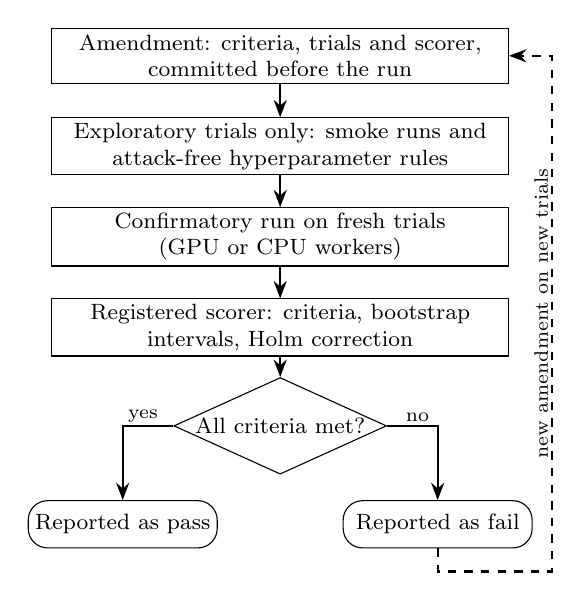
\begin{tikzpicture}[x=1cm,y=1cm]
\node[box, minimum width=58mm] (a) at (3.3,0) {Amendment: criteria, trials and scorer,\\committed before the run};
\node[box, minimum width=58mm] (b) at (3.3,-1.15) {Exploratory trials only: smoke runs and\\attack-free hyperparameter rules};
\node[box, minimum width=58mm] (c) at (3.3,-2.3) {Confirmatory run on fresh trials\\(GPU or CPU workers)};
\node[box, minimum width=58mm] (d) at (3.3,-3.45) {Registered scorer: criteria, bootstrap\\intervals, Holm correction};
\node[dec] (e) at (3.3,-4.7) {All criteria met?};
\node[term, minimum width=24mm] (p) at (1.3,-5.95) {Reported as pass};
\node[term, minimum width=24mm] (f) at (5.3,-5.95) {Reported as fail};
\draw[arr] (a) -- (b);
\draw[arr] (b) -- (c);
\draw[arr] (c) -- (d);
\draw[arr] (d) -- (e);
\draw[arr] (e.west) -| node[lab, above, pos=0.3]{yes} (p.north);
\draw[arr] (e.east) -| node[lab, above, pos=0.3]{no} (f.north);
\draw[darr] (f.south) -- (5.3,-6.55) -- (6.75,-6.55) -- node[lab, sloped, above, pos=0.5]{new amendment on new trials} (6.75,0) -- (a.east);
\end{tikzpicture}
\caption{Pre-registered evaluation protocol. A failed criterion is reported as a failure; a design change is tested only under a new amendment on new trials. Solid arrows give the order of the steps; the dashed arrow is the path taken after a failure.}
\label{fig:protocol}
\end{figure}

%======================================================================
\section{Results}\label{sec:results}
\subsection{Certificate Soundness}
Across all confirmatory result files, 1,080,120 rows were recorded, of which 233,870 carry a certificate inside the threat model; none violates its certificate or its action certificate. The 179 violations recorded outside the threat model occur exactly where they were predicted in advance: in the ablation that adds momentum to the promoted tier (80 runs, drift up to 2.13 times the bound) and when the adversaries outnumber the assumed $f$ (99 runs). The bound is tight: in the witness experiment the largest ratio of measured drift to certificate is 0.999.

\subsection{Witness Complexity}\label{sec:witness}
Table~\ref{tab:witness} reports the smallest number of honest witnesses at which each defence serves a fact (clean recall at least 0.5 at that and every larger value), from 26,550 Tier-A runs. The thresholds equal $2f+1$ for \TabC\ and $f+1$ for \TabW\ in all six configurations, as Theorem~\ref{thm:witness} predicts, while the trimmed mean, median, geometric median and RobustRAG need 6, 11, 21 and 41--60 witnesses for $n=10,20,40,80$ (Fig.~\ref{fig:witness}). Titans and TMA-NM serve facts with one to seven witnesses but were forged in every configuration; both Tabayyun variants recorded no installation, no flip and no amnesia at any served $m$ under all four attacks.

\begin{table}[!t]
\caption{Witness Threshold $m^\star$: Honest Witnesses Needed Before a Fact Is Served (Tier A, Seeds 1000--1009). Titans and TMA-NM Were Forged in Every Configuration}
\label{tab:witness}
\centering\footnotesize
\setlength{\tabcolsep}{3pt}
\resizebox{\columnwidth}{!}{%
\begin{tabular}{@{}cc|cc|cccc|cc|cc@{}}
\toprule
$n$ & $f$ & Titans & TMA & TrM. & Med. & GeoM. & RRAG & \TabC & \TabW & $f{+}1$ & $2f{+}1$ \\
\midrule
\inputtab{data/tab_witness.tex}
\bottomrule
\end{tabular}}
\end{table}

\begin{figure}[!t]
\centering
\begin{tikzpicture}
\begin{axis}[width=\columnwidth, height=50mm, xmode=log, log basis x=2, xtick={10,20,40,80}, xticklabels={10,20,40,80},
  xlabel={Number of sources $n$ ($f=2$)}, ylabel={Witness threshold $m^\star$}, ymin=0, ymax=64,
  legend style={font=\scriptsize, at={(0.5,-0.32)}, anchor=north, draw=black, fill=white, legend columns=2}, legend cell align=left,
  tick label style={font=\footnotesize}, label style={font=\footnotesize}, grid=major, grid style={gray!30}]
\addplot[black, thick, mark=square*] table[x=n, y=trmean] {data/witness_f2.dat};
\addlegendentry{Trimmed mean}
\addplot[black, thick, densely dashed, mark=triangle*] table[x=n, y=median] {data/witness_f2.dat};
\addlegendentry{Median, geo.\ median, RobustRAG}
\addplot[black, thick, mark=o] table[x=n, y=tabc] {data/witness_f2.dat};
\addlegendentry{\TabC\ ($2f+1=5$)}
\addplot[black, thick, mark=*] table[x=n, y=tabw] {data/witness_f2.dat};
\addlegendentry{\TabW\ ($f+1=3$)}
\addplot[gray, dotted, thick, domain=10:80, samples=2] {x/2};
\addlegendentry{$n/2$}
\end{axis}
\end{tikzpicture}
\caption{Witness threshold against the number of sources (Tier A, $f=2$, 10 seeds per point). The Tabayyun thresholds stay at $2f+1$ and $f+1$; majority aggregators follow $n/2$ or more.}
\label{fig:witness}
\end{figure}

\subsection{Recall and Security Under the Static Protocol}
Table~\ref{tab:static} reports clean recall in the dense and locality regimes, the worst installed rate over the static attacks and cells, and the fraction of certified and correct tokens, for the three trained models (Tier B) and the two pretrained models (Tier D), 100 trials per cell. \TabW\ recalls 0.83 (Tier B) and 0.82 (Tier D) of locally held facts, 32 to 34 points more than \TabC\ on every model, with a worst installed rate of 0.020 and 0.005. Its recall follows (\ref{eq:recall}) with $k=f+1$ within 0.10 in 80 of 80 model--cell combinations, and that of \TabC\ with $k=2f+1$ in 79 of 80. Krum and the RobustRAG port are secure but recall at most 0.41 of local facts. Fig.~\ref{fig:recalllaw} compares the measured recall of both variants with (\ref{eq:recall}); the largest deviation is 0.042 for \TabW\ and 0.101 for \TabC.

\begin{figure}[!t]
\centering
\begin{tikzpicture}
\begin{axis}[width=0.86\columnwidth, height=0.80\columnwidth, xmin=0, xmax=1.02, ymin=0, ymax=1.02,
  xlabel={Predicted recall, (\ref{eq:recall})}, ylabel={Measured clean recall},
  legend style={font=\scriptsize, at={(0.97,0.03)}, anchor=south east, draw=black, fill=white}, legend cell align=left,
  tick label style={font=\footnotesize}, label style={font=\footnotesize}, grid=major, grid style={gray!30}]
\addplot[gray!60, fill=gray!15, draw=none, forget plot] coordinates {(0,0.1) (0.92,1.02) (1.02,1.02) (1.02,0.92) (0.1,0) (0,0) (0,0.1)};
\addplot[black, thin, domain=0:1.02, samples=2, forget plot] {x};
\addplot[only marks, mark=o, mark size=1.6pt, black] table[x=pred, y=meas, discard if not={variant}{C}] {data/recall_law.dat};
\addlegendentry{\TabC, $k=2f+1$}
\addplot[only marks, mark=*, mark size=1.3pt, black] table[x=pred, y=meas, discard if not={variant}{W}] {data/recall_law.dat};
\addlegendentry{\TabW, $k=f+1$}
\end{axis}
\end{tikzpicture}
\caption{Recall law. Each point is one model--cell combination (5 models, 16 cells, 100 trials). The shaded band marks a deviation of at most 0.10 from (\ref{eq:recall}); 80 of 80 points of \TabW\ and 79 of 80 points of \TabC\ lie inside it.}
\label{fig:recalllaw}
\end{figure}

The comparison is not uniformly favourable. When every honest source knows every fact, the trimmed mean, median and geometric median recall 0.96--0.97 against 0.93--0.94 for \TabW\ under these attacks, and \TabW\ is Pareto-dominated in 4 of 16 cells on Qwen2.5-1.5B and 5 of 16 on GPT-2 XL, all of them dense or well observed; on the three Tier-B models it is non-dominated in 48 of 48 cells. The same aggregators are installed on 27--47\% of targets by the static attacks and are broken further by adaptive attacks (Section~\ref{sec:adaptive}).

\begin{table*}[!t]
\caption{Static Protocol, Tiers B and D (Trials 1100--1199, 16 Cells per Model). Recall: Mean Clean Recall Over Dense or Locality Cells and Models; Inst.: Worst Installed Rate Over Attacks, Cells and Models (Lower Is Better); Cert.: Mean Fraction of Tokens Certified and Correct}
\label{tab:static}
\centering\footnotesize
\begin{tabular}{@{}l|cccc|cccc@{}}
\toprule
 & \multicolumn{4}{c|}{Tier B: MemLM d128 / d256 / d512} & \multicolumn{4}{c}{Tier D: GPT-2 XL / Qwen2.5-1.5B} \\
Defence & Recall dense $\uparrow$ & Recall locality $\uparrow$ & Inst.\ $\downarrow$ & Cert.\ $\uparrow$ & Recall dense $\uparrow$ & Recall locality $\uparrow$ & Inst.\ $\downarrow$ & Cert.\ $\uparrow$ \\
\midrule
\inputtab{data/tab_static.tex}
\bottomrule
\end{tabular}
\end{table*}

\subsection{Adaptive Attacks}\label{sec:adaptive}
Table~\ref{tab:worst} reports, for each defence, the worst installed rate over the static attacks, the gradient attack and the union attacker, and the maximum over all three. The gradient attack installs the attacker's value on 100\% of targets in some Tier-B cells for the trimmed mean and the geometric median, and on 70--83\% on Tier D (88\% for the trimmed mean under the union attacker). \TabC\ reaches 0.283 on Tier B: in the thinnest cell ($f=3$, $\rho=0.4$, $R=1$) the target is rarely promoted, its read is close to zero, and a bounded push through cross-talk from other promoted directions decides the token. \TabW\ promotes such facts on $f+1$ witnesses and is installed on at most 0.050 of targets on Tier B and 0.005 on Tier D. Fig.~\ref{fig:union} shows the union attack per model, and Fig.~\ref{fig:tradeoff} places every defence of Tier D in the plane of local recall and worst-case installation.

\begin{figure}[!t]
\centering
\begin{tikzpicture}
\begin{axis}[width=0.95\columnwidth, height=58mm, xmin=-0.04, xmax=1.0, ymin=-0.06, ymax=1.08,
  xlabel={Worst installed rate over every attack run}, ylabel={Clean recall, locality cells},
  legend style={font=\scriptsize, at={(0.5,-0.25)}, anchor=north, legend columns=2, draw=black, fill=white},
  tick label style={font=\footnotesize}, label style={font=\footnotesize}, grid=major, grid style={gray!30},
  nodes near coords, point meta=explicit symbolic, every node near coord/.style={font=\scriptsize, inner sep=2pt}]
\addplot[only marks, mark=*, mark size=1.8pt, black, visualization depends on={value \thisrow{anchor}\as\anc},
  every node near coord/.append style={anchor=\anc}] table[x=x, y=y, meta=label] {data/tradeoff_D_adapt.dat};
\addlegendentry{static, gradient and union attacks}
\addplot[only marks, mark=o, mark size=1.8pt, black, visualization depends on={value \thisrow{anchor}\as\anc},
  every node near coord/.append style={anchor=\anc}] table[x=x, y=y, meta=label] {data/tradeoff_D_static.dat};
\addlegendentry{static attacks only}
\end{axis}
\end{tikzpicture}
\caption{Recall and security on Tier D (GPT-2 XL and Qwen2.5-1.5B). Recall is the mean over the eight locality cells and both models; the horizontal axis is the worst installed rate over every attack run for that defence (Table~\ref{tab:worst} for the filled markers). C0, C and W denote \TabC0, \TabC\ and \TabW.}
\label{fig:tradeoff}
\end{figure}

Under certify-or-abstain serving and the union attacker, \TabW\ served no wrong token in any cell and \TabC\ served one in 60 targets in one cell; under the static attacks of Table~\ref{tab:static}, \TabW\ served one wrong token in 200 targets in its worst Tier-D cell and none on Tier B. \TabW\ also lost the true fact less often under the union attack (mean amnesia 0.125--0.133 against 0.342--0.350 for \TabC) and served 45--61\% of attacked facts with a correct certified token, against 1--6\% for \TabC.

\begin{table}[!t]
\caption{Worst Installed Rate Over Every Attack Run (Static; Gradient: PGD With Straight-Through Gate; Union: Union Attacker; --: Not Run)}
\label{tab:worst}
\centering\footnotesize
\setlength{\tabcolsep}{3pt}
\resizebox{\columnwidth}{!}{%
\begin{tabular}{@{}l|cccc|cccc@{}}
\toprule
 & \multicolumn{4}{c|}{Tier B} & \multicolumn{4}{c}{Tier D} \\
Defence & Stat. & Grad. & Union & Max & Stat. & Grad. & Union & Max \\
\midrule
\inputtab{data/tab_worst.tex}
\bottomrule
\end{tabular}}
\end{table}

\begin{figure}[!t]
\centering
\begin{tikzpicture}
\begin{axis}[width=0.95\columnwidth, height=46mm, ybar, bar width=6pt, enlarge x limits=0.25,
  symbolic x coords={d128,d256,d512}, xtick=data, xticklabels={MemLM d128,MemLM d256,MemLM d512},
  ylabel={Worst installed rate}, ymin=0, ymax=1.1,
  legend style={font=\scriptsize, at={(0.5,1.03)}, anchor=south, legend columns=2, draw=black, fill=white}, legend cell align=left,
  tick label style={font=\footnotesize}, label style={font=\footnotesize}, ymajorgrids, grid style={gray!30}]
\addplot[draw=black, fill=black] table[x=model, y=trmean] {data/union_tierB.dat};
\addlegendentry{Trimmed mean}
\addplot[draw=black, fill=gray!55] table[x=model, y=tabc0] {data/union_tierB.dat};
\addlegendentry{\TabC0}
\addplot[draw=black, pattern=north east lines] table[x=model, y=tabc] {data/union_tierB.dat};
\addlegendentry{\TabC}
\addplot[draw=black, fill=white] table[x=model, y=tabw] {data/union_tierB.dat};
\addlegendentry{\TabW}
\end{axis}
\end{tikzpicture}
\caption{Union attacker on Tier B (trials 360--389, 16 cells per model): worst installed rate over cells. \TabW\ stays at or below 0.050 on all three models.}
\label{fig:union}
\end{figure}

\subsection{Capacity and Sharding}\label{sec:scale}
Fig.~\ref{fig:scale} reports the GPT-2 XL memory with $d_k=1024$ and $F$ facts per memory. Without sharding, certified and correct tokens fall from 0.96--1.00 at $F\le 16$ to 0.04--0.05 at $F=256$ and 0 at $F=1024$, and uncertified answers become attackable (worst installed 0.15--0.45 at $F=256$). Interference between near-orthogonal keys grows with $F/d_k$, honest quarantines disagree, and the certificate widens; certify-or-abstain still served no wrong token at any $F$, but it served almost nothing beyond $F=64$. With 32 facts per shard (\ref{eq:shard}), certified and correct tokens stay at 0.90--0.94 for \TabC\ and 0.95--1.00 for \TabW\ up to $F=1024$, with no installation and no violation. The cost of the gate and certificate grows linearly, from 0.036\,s to 2.27\,s per promotion round between $F=16$ and $F=1024$, about 13 times the trimmed mean at $F=1024$.

\begin{figure}[!t]
\centering
\begin{tikzpicture}
\begin{groupplot}[group style={group size=2 by 1, horizontal sep=13mm}, width=0.54\columnwidth, height=42mm,
  xmode=log, log basis x=2, xtick={16,64,256,1024}, xticklabels={16,64,256,1024}, xlabel={Facts per memory $F$},
  tick label style={font=\scriptsize}, label style={font=\footnotesize}, title style={font=\footnotesize}, grid=major, grid style={gray!30}]
\nextgroupplot[ylabel={Certified and correct}, ymin=-0.05, ymax=1.08, title={(a) Certification},
  legend to name=scaleleg, legend columns=4, legend style={font=\scriptsize, draw=black, fill=white}, legend cell align=left]
\addplot[black, thick, densely dashed, mark=o] table[x=F, y=ccCflat] {data/scaling.dat};
\addlegendentry{C, one memory}
\addplot[black, thick, densely dashed, mark=*] table[x=F, y=ccWflat] {data/scaling.dat};
\addlegendentry{W, one memory}
\addplot[black, thick, mark=o] table[x=F, y=ccCshard] {data/scaling.dat};
\addlegendentry{C, sharded}
\addplot[black, thick, mark=*] table[x=F, y=ccWshard] {data/scaling.dat};
\addlegendentry{W, sharded}
\nextgroupplot[ylabel={Worst installed}, ymin=-0.02, ymax=0.5, title={(b) Security}]
\addplot[black, thick, densely dashed, mark=o] table[x=F, y=instCflat] {data/scaling.dat};
\addplot[black, thick, densely dashed, mark=*] table[x=F, y=instWflat] {data/scaling.dat};
\addplot[black, thick, mark=o] table[x=F, y=instCshard] {data/scaling.dat};
\addplot[black, thick, mark=*] table[x=F, y=instWshard] {data/scaling.dat};
\end{groupplot}
\end{tikzpicture}\\[1mm]
\pgfplotslegendfromname{scaleleg}
\caption{Capacity on Tier D (GPT-2 XL, $d_k=1024$, 10 trials per point). (a) Certified and correct tokens in the two well-observed cells; (b) worst installed rate over all cells and static attacks. Dashed: one memory; solid: 32 facts per shard.}
\label{fig:scale}
\end{figure}

\subsection{Federation and Radio Access Network Control}
Table~\ref{tab:fedoran} summarizes the federated tier (5,600 runs) and the ColO-RAN tier (10,400 runs), both with the cone gate. Averaging promoted client memories (FedAvg) was flipped in every cell, and federated averaging over ungated Titans clients installed the attacker's value in every cell. Server-side trimmed mean, median and geometric median kept the attacker out but forgot the attacked fact in up to 85\% of trials when it was held by a minority of clients; two-level Tabayyun recorded no flip, no amnesia and no violation of (\ref{eq:fed}) in 800 runs. In the slicing controller the worst final-epoch hijack rate of \TabC\ was 0.05 against 1.00 for Titans and 0.90 for the trimmed mean, and 88.8\% of clean decisions were certified to be within 10\% of the optimal utility by (\ref{eq:regret}). The registered criterion of non-domination failed in 3 of 8 cells: in the dense cells the trimmed mean, median and RobustRAG were equally secure with a regret lower by at most 0.028 on a utility range of 1.88.

\begin{table}[!t]
\caption{Federated Tier (Left; Locality Recall, Worst Flip and Amnesia) and ColO-RAN Slicing (Right; Worst Hijack, Mean Clean Regret, Worst Regret)}
\label{tab:fedoran}
\centering\footnotesize
\setlength{\tabcolsep}{2.4pt}
\begin{tabular}{@{}lccc@{}}
\toprule
Server rule & Rec.\ $\uparrow$ & Flip $\downarrow$ & Amn.\ $\downarrow$ \\
\midrule
\inputtab{data/tab_fed.tex}
\bottomrule
\end{tabular}\\[4pt]
\begin{tabular}{@{}lccc@{}}
\toprule
Controller memory & Hijack $\downarrow$ & Regret $\downarrow$ & Worst reg.\ $\downarrow$ \\
\midrule
\inputtab{data/tab_oran.tex}
\bottomrule
\end{tabular}
\end{table}

\subsection{Ablations and Limits}\label{sec:ablation}\label{sec:limits}
\emph{Momentum.} Momentum $0.5$ or $0.9$ in the promoted tier broke the certificate in 40 of 200 runs each, with drift up to 1.45 and 2.13 times the bound. \emph{Cone test.} Removing it kept the certificate sound and the installed rate at 0, but made the bound 20 times looser (Frobenius norm 4.62 against 0.23). \emph{Unique facts.} Facts known to one source are never served by the certified read; their owner still reads them from its own quarantine. Under Dirichlet(0.1) observation rates \TabC\ kept 0.70 recall, against 0.04--0.05 for the trimmed mean, median and RobustRAG. \emph{More adversaries than assumed.} With $f=2$ assumed and 3 or 4 actual adversaries the certificate was violated in a third of the runs, but the fact was neither flipped nor erased; with 5 adversaries, which equals $2f+1$, every defence failed. \emph{Correlated sources.} When three honest sources relayed a poisoned upstream feed, so that adversaries and relays together reached $k$, the attacked fact was installed in 35\% of runs with no certificate violation: the certificate bounds deviation from the honest consensus, not from the truth.

%======================================================================
\section{Discussion}\label{sec:discussion}
The results separate what corroboration buys from what it cannot. The certificate is sound in every run inside the threat model, and its scope is precise: it bounds the deviation from the mean of the honest corroborators under the same promotion decisions. It does not certify truth, and it assumes that honest sources are independent and that at most $f$ sources are Byzantine; Section~\ref{sec:limits} shows the failure when either assumption is removed.

The advantage over robust aggregation is a statement about witnesses. When every honest source knows a fact, majority aggregators serve it with slightly higher recall under static attacks, and the method adds only the certificate; they are, however, installed on 70--100\% of targets by gradient attacks. When knowledge is local, Theorem~\ref{thm:witness}(d) forces majority aggregators to forget, and the Tabayyun thresholds are independent of $n$. The agreement gate trades a bounded shift of up to $2\epsilon\sigma_u$ on facts with fewer than $2f+1$ witnesses for a lower threshold; the union attacks did not exploit that room beyond 5\% of targets, but no proof excludes a stronger combinatorial attack on the choice of corroborators.

Four further limits apply. The certified tier has a capacity of about $d_k/16$ facts per memory, removed by sharding at a cost that grows linearly with the number of facts. The memory of Tier D sits at the input of the unembedding of a frozen model, which makes the action certificate exact; a memory inside the network would require a Lipschitz form of (\ref{eq:action}). The agreement tolerance $\epsilon$ was calibrated per tier and per load on attack-free data. Liveness under denial-of-promotion attacks was measured, not proved.

%======================================================================
\section{Conclusion}\label{sec:conclusion}
This paper presented a two-tier test-time memory in which sources write into separate quarantines and facts enter a shared, linear tier only after corroboration, with a per-query runtime certificate that is instance-optimal. The witness analysis shows that $f+1$ agreeing witnesses are necessary and sufficient for bounded error and $2f+1$ for range validity, independently of the number of sources, while majority aggregation needs more than half of them. In pre-registered experiments on five substrates no certificate was violated inside the threat model; the agreement-gated variant was installed on at most 5.0\% of targets under gradient and union attacks, recalled 32--34 points more locally held facts than the cone-gated variant, and remained certified up to 1,024 facts per memory with sharding. Future work includes certificates for memories inside the network, a proof of liveness, and tests on real multi-source deployments.

\section*{Data and Code Availability}
Code, configurations, the pre-registration with its 18 amendments, all result files and the script that regenerates every number, table and figure of this paper are available at \url{https://github.com/Abraheem13/tabayyun-cert}. CounterFact, ColO-RAN and the pretrained models are publicly available.

\bibliographystyle{IEEEtran}
\bibliography{refs}

\end{document}
